\documentclass[aspectratio=1610,20pt,utf8]{beamer}
\setbeamersize{text margin left=5pt,text margin right=5pt}
\setbeamerfont{subsection in toc}{size=\small}
\usepackage[utf8]{inputenc}
\usepackage[T1]{fontenc}
\usepackage[USenglish]{babel}
\usepackage{graphicx} % graphics
\usepackage{array, tabularx, caption, boldline}
\usepackage{mathabx}
\usepackage{mathpazo}
\usepackage{eulervm}
\usepackage{tikz} %for the points
\usepackage{amssymb}
\usepackage{enumitem}
\setlistdepth{30}
\setlist[itemize]{label=\textbullet}

\newcommand{\shrug}[1][]{%
	\begin{tikzpicture}[baseline,x=0.8\ht\strutbox,y=0.8\ht\strutbox,line wid2th=0.125ex,#1]
	\def\arm{(-2.5,0.95) to (-2,0.95) (-1.9,1) to (-1.5,0) (-1.35,0) to (-0.8,0)};
	\draw \arm;
	\draw[xscale=-1] \arm;
	\def\headpart{(0.6,0) arc[start angle=-40, end angle=40,x radius=0.6,y radius=0.8]};
	\draw \headpart;
	\draw[xscale=-1] \headpart;
	\def\eye{(-0.075,0.15) .. controls (0.02,0) .. (0.075,-0.15)};
	\draw[shift={(-0.3,0.8)}] \eye;
	\draw[shift={(0,0.85)}] \eye;
	% draw mouth
	\draw (-0.1,0.2) to [out=15,in=-100] (0.4,0.95); 
	\end{tikzpicture}}
\newcommand*\circled[1]{\tikz[baseline=(char.base)]{\node[shape=circle,draw,inner sep=2pt] (char) {#1};}}

\usetheme{unipassau}


% title slide definition
\title[Team Hams]{Sprint 05}
\subtitle{Bugfixing \\(Implementation)}
\author[\today]{Benedikt Holler}
\institute[Team Hams]
{
  Team Hams\\
  Leading Product Owner and Scrum Master\\
}
\date{25.01.2018}

%--------------------------------------------------------------------
%                            Titlepage
%--------------------------------------------------------------------

\begin{document}

\begin{frame}[plain]
  \titlepage
\end{frame}

\begin{frame}{Overview}
\begin{itemize} \small
	\item Sprint
	\begin{itemize} \tiny
		\item Burndown
		\item Mistakes
	\end{itemize}
	\item Product
	\begin{itemize} \tiny
		\item Major Changes
		\item Known issues
		\item Live Demo
	\end{itemize}
	\item Documentation
	\begin{itemize} \tiny
		\item Security Report
		\item Unit Tests
		\item Manual Tests
		\item Bug Report
		\item Manuals
	\end{itemize}
	\item What we learned
\end{itemize}	
%\tableofcontents
\end{frame}

%-------------------------------------------------------------------
%                            Content
%-------------------------------------------------------------------
%%%%%%%%%%%%%%%%%%%%%%%%%%%%%%%%%%%%%%%%%%%%%%%%%%%%%%%%%%%%%%%%%%%%%%
\section{Sprint} 
%--------------------------------------------------------------------%

\subsection{Burndown}
\begin{frame}{Burndown Jira}
	\centering
	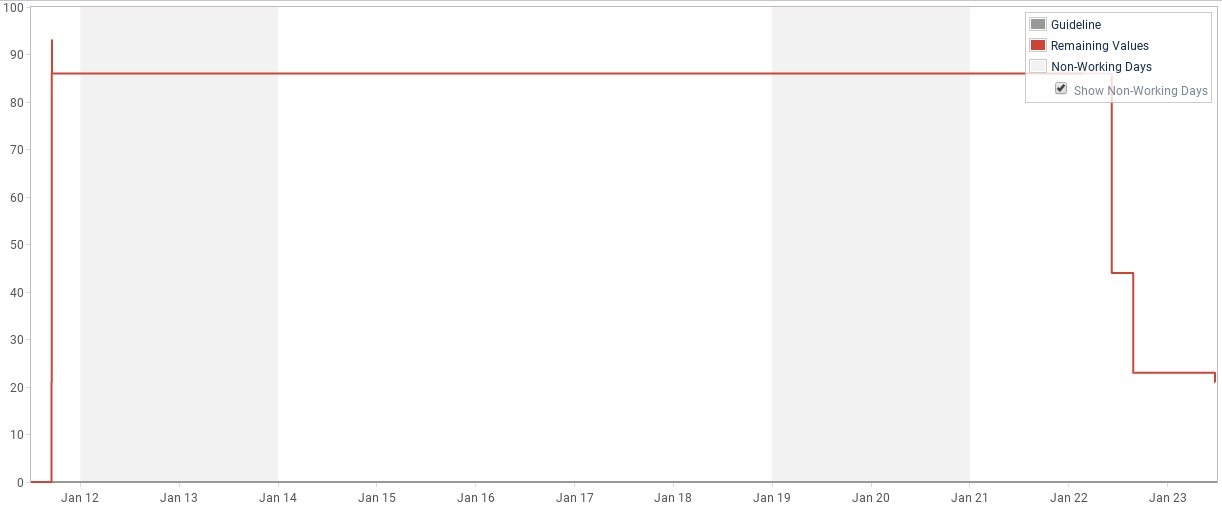
\includegraphics[width=15cm]{img/s05_hams_jira_burndown.jpg}
\end{frame}

\subsection{Mistakes}
\begin{frame}{Mistakes}
 \itemize
 \item Testing and bugfixing began before actual finalization of the product
 \item Major code changes in the middle of the sprint led to conflicts
 \item Very late deployment: Problems occured while running on VM that were not present on local build
 
\end{frame}
%%%%%%%%%%%%%%%%%%%%%%%%%%%%%%%%%%%%%%%%%%%%%%%%%%%%%%%%%%%%%%%%%%%%%%
\section{Product}
\begin{frame}
\frametitle{Major changes}
\itemize
\item Dashboards and Management Pages are functional
\item Overworked Alert Rules (Average, Standard Deviation, Kurtosis)
\item No more temporary links for password distribution/reset (Vue limitation)
\item Currently deployed version is not version in the final submission (fixes were done)
\end{frame}
\begin{frame}
\frametitle{Known issues}
\itemize
\item No KPI records older than 60 minutes are displayed on dashboard
\item FE slows down heavily over time (Probably gumming up browser cache)
\end{frame}
\begin{frame}
\frametitle{Live Demo}
\itemize
\item Dashboard
\item User creation and changes
\item User rights
\end{frame}

%%%%%%%%%%%%%%%%%%%%%%%%%%%%%%%%%%%%%%%%%%%%%%%%%%%%%%%%%%%%%%%%%%%%%%
\section{Documentation}

\subsection{Security Report}
\begin{frame}
\frametitle{Security Report}
\itemize
\item Port scan with nmap: Weak cipher key length
\item Automated scans with nikto and owasp-zap: Slight clickjacking vulnerability, Email address could be detected in SSL info
\end{frame}
\begin{frame}
\frametitle{Security Report}
\itemize
\item Burp Proxy: Capture requests of user interactions, check jwt-accesstoken
\item Wireshark: Encryption could be verified
\item SQL injection: No vulnerability found (SQL queries are auto-generated by Spring)
\item Brute Force Login: Very weak password policy
\end{frame}

%%%%%%%%%%%%%%%%%%%%%%%%%%%%%%%%%%%%%%%%%%%%%%%%%%%%%%%%%%%%%%%%%%%%%%

\subsection{Unit Tests}
\begin{frame}
\frametitle{Unit Tests}
\begin{itemize}
	\item Halfway through the sprint, all Unit Tests were written and "green". \\
	\item However, major code changes broke most Unit Tests. \\
    \item Re-writing Unit Tests was not possible due to limited time.
\end{itemize}
\end{frame}

%%%%%%%%%%%%%%%%%%%%%%%%%%%%%%%%%%%%%%%%%%%%%%%%%%%%%%%%%%%%%%%%%%%%%%
\subsection{Manual Tests}
\begin{frame}
\frametitle{Manual Tests}
\begin{center}
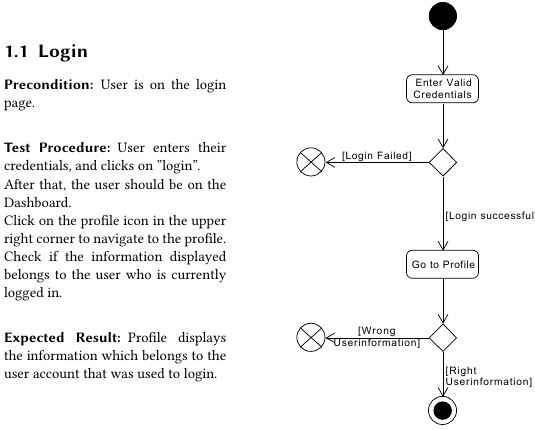
\includegraphics[height=200px]{tests.jpg}
\end{center}
\end{frame}

%%%%%%%%%%%%%%%%%%%%%%%%%%%%%%%%%%%%%%%%%%%%%%%%%%%%%%%%%%%%%%%%%%%%%%

\subsection{Bug Report}
\begin{frame}
\frametitle{Bug Report}
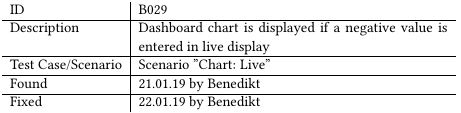
\includegraphics{bug01.jpg}
\end{frame}

\begin{frame}
\frametitle{Bug Report}
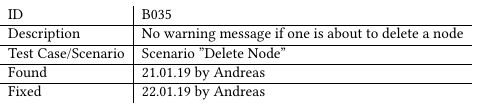
\includegraphics{bug02.jpg}
\end{frame}

\begin{frame}
\frametitle{Bug Report}
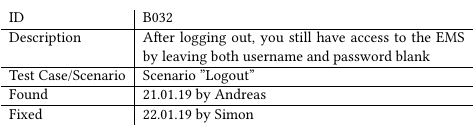
\includegraphics{bug03.jpg}
\end{frame}

\begin{frame}
\frametitle{Bug Report}
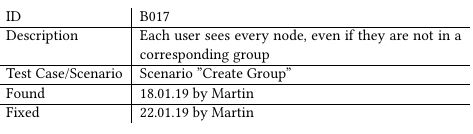
\includegraphics{bug04.jpg}
\end{frame}

\begin{frame}
\frametitle{Bug Report}
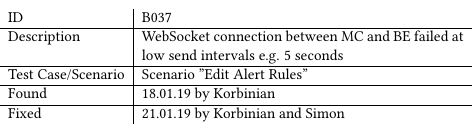
\includegraphics{bug05.jpg}
\end{frame}


%%%%%%%%%%%%%%%%%%%%%%%%%%%%%%%%%%%%%%%%%%%%%%%%%%%%%%%%%%%%%%%%%%%%%%

\subsection{Manuals}
\begin{frame}
\frametitle{Manuals}
\begin{itemize}
\item User Manual: Intended to be readable by a "Luser" :) 
\item MC Manual: Advanced manual with instructions on how to set up a MC on a device
\end{itemize}
\end{frame}

%%%%%%%%%%%%%%%%%%%%%%%%%%%%%%%%%%%%%%%%%%%%%%%%%%%%%%%%%%%%%%%%%%%%%%
\section{Sprint retrospective and EP Wrap-up}
\subsection{Sprint 05: Negative}
\begin{frame}
\frametitle{Sprint 05: Negative}
\begin{itemize}
\item workload left from Sprint 04 caused a major delay
\item Testing was started too soon (in our specific case)
\item Deployment began too late
\end{itemize}
\end{frame}

%%%%%%%%%%%%%%%%%%%%%%%%%%%%%%%%%%%%%%%%%%%%%%%%%%%%%%%%%%%%%%%%%%%%%%

\subsection{Sprint 05: Positive}
\begin{frame}
\frametitle{Sprint 05: Positive}
\begin{itemize} 
	\item Great implementation catch-up during the first half of the sprint
	\item No panic despite pressing time constraints
	\item After major roadblocks, we still delivered a presentable product!
	\end{itemize}
\end{frame}

\subsection{EP Wrap-Up}
\begin{frame}\small
\begin{itemize}
	\frametitle{EP Wrap-Up}
	\item Across the entire project, we were prone to underestimating our tasks
	\item Communication was generally lacking, mostly due to different schedules)
	\item But in the end: Teamwork makes the dream work!
	\item Final standings: 12,000 Lines of Code (6,000 Backend, 4,000 Frontend, 2,000 Monitoring Client) across 1,000 commits
	\end{itemize}
\end{frame}
\end{document}
